\documentclass{paper}


\usepackage[utf8]{inputenc}

\usepackage{circledsteps}

\usepackage[english]{babel}
\usepackage[a4paper, margin=0.8in]{geometry}

\usepackage{parskip}

\usepackage{amsthm}
\usepackage{amssymb}
\usepackage{amsmath}

\usepackage{float}
\usepackage{graphicx} 

% variables you can adjust
\newcommand{\titleVar}{\large Seminar Report on\\ \LARGE TCUDB: Accelerating Database with Tensor Processors \\{\large {by Yu-Ching Hu, Yuliang Li, Hung-Wei Tseng}}
}

% end variables you can adjust


% last configuration before document starts
\title{\titleVar}
\author{David R. Zollikofer\\ ETH Zürich}
\date{\today}



\usepackage{mathpazo}

% optional math environments



\begin{document}
	
\twocolumn[\maketitle 
\hrule 

\begin{abstract}Recent advances in hardware accelerators for matrix multiplications have massively sped up deep learning workflows. In this seminar report we will outline how NVIDIAs Tensor Cores can be used to speed up database workloads; for this we will take a close look at the framework presented in \cite{hu2021tcudb}, analyze it, compare it to other relevant literature \cite{he2022query}. Last but not least we will also highlight shortcomings of the presented approaches and give a short outlook.
\end{abstract}

\hrule\bigskip
]

	

\section{Introduction}
The introduction of Tensor Cores for NVIDIA GPUs has resulted significant speed improvements for matrix multiplication heavy workflows \cite{markidis2018nvidia}. Although primarily used for deep learning thanks their CUDA API they can easily be employed for a plethora of different applications. The paper "Accelerating Database with Tensor Processors" by Yu-Ching Hu, Yuliang Li, Hung-Wei Tseng \cite{hu2021tcudb} presents a novel framework to use Tensor Cores for database acceleration.
	
	\section{Using Tensor Cores to Accelerate Databases}
	
	\subsection{The Tensor Abstraction}
	Databases inherently being very flexible in the data they represent. Matrices as used by the Tensor Cores on NVIDIA GPUs however have are limited to 16-bit floating point precision. A key challenge is mapping database primitives as well as operators to these tensors.
	
	\subsection{Mapping Database Operators to Tensor Operations}
	
	The paper \cite{hu2021tcudb} treats this transformation rather theoretical; instead of a full theoretical treatment we follow an example driven presentation here.
	
	Assume we are given 
	
	\subsection{End-to-End Pipeline}
	
	Running computations on tensor cores does not come without cost, from data movement and transformation over to precision constraints, present challenges for a competitive database system. In TCUDB the authors acknowledge these limitations of tensor core based processing and present a workflow as depicted in Figure \ref{fig:pipeline}.

	First the query is analyzed \Circled{1} and it is pattern matched whether it contains operators which can be accelerated using the presented approach. Whenever this or one of the following test fails TCUDB resorts to standard processing not using tensor cores. In \Circled{2} TCUDB checks wether the data as well as results will fit into the limited precision, to help this analysis TCUDB stores minimum, maximum and mean values for any table columns.
	
	As the presented transformation results in sparse matrices if there are many TODO TCUDB decides in \Circled{3} if a sparse or dense matrix multiplication should be used. As GPU memory is limited TCUDB also needs to ensure that \Circled{4} TODO
	
	\begin{figure}[h]
		\centering
		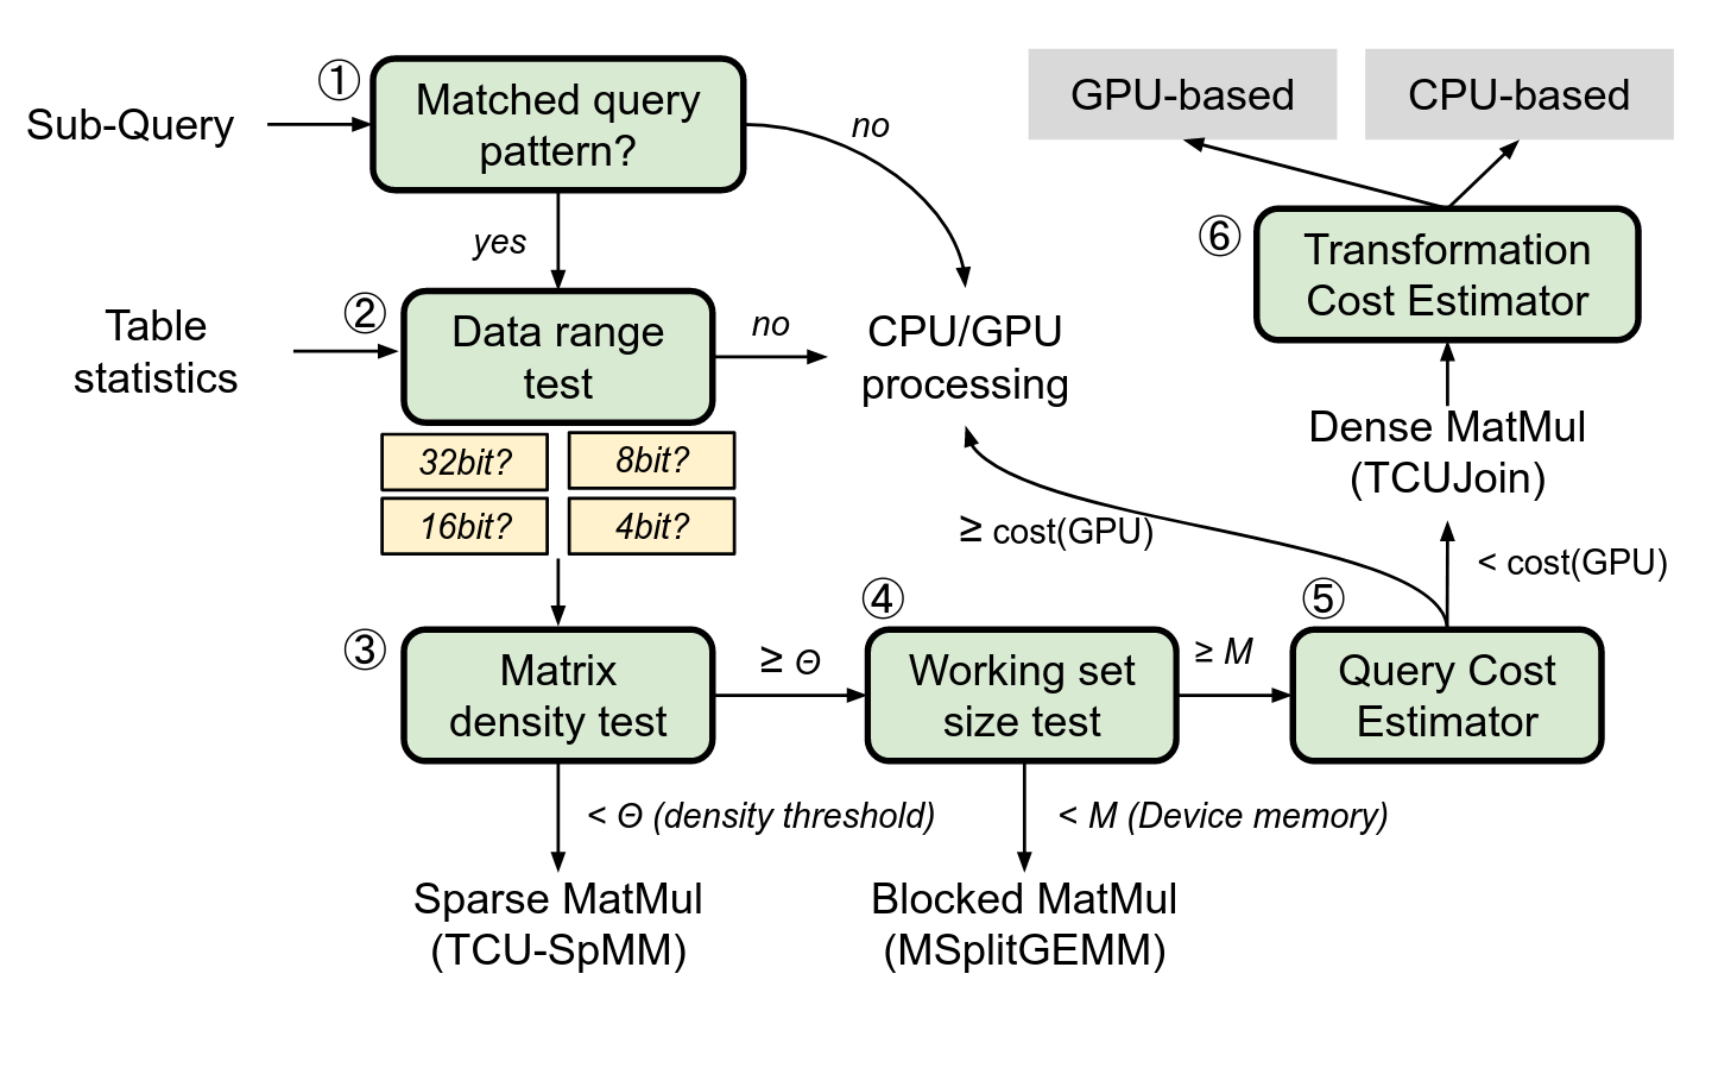
\includegraphics[width=0.9\linewidth]{pipeline}
		\caption{The workflow of the TCUDB query optimizer. Figure from \cite{hu2021tcudb}.} 
		\label{fig:pipeline}
	\end{figure}
	
	\section{Comparison to Related Work} \label{sec:rel_work}
	As tensor processors are quite a new development there is little other literature to compare the "Accelerating Database with Tensor Processors" paper to. 
	
	The authors of TCUDB have chosen to compare their approach to MonetDB, a commercial column-based database primarily used for data warehousing, as well as  Yinyang DB \cite{yuan2013yin}, a database acceleration framework using CUDA cores aimed at data warehousing workloads. 
	
	Although these approaches are used as a benchmark for TCUDB they do not use tensor cores and are hence further discussed in Section \ref{sec:perf_eval} on performance evaluation.
	
	A paper also using Tensor Cores for database acceleration is "Query Processing on Tensor Computation Runtimes" (TQP) \cite{he2022query} by He et al. which was released about half a year after TCUDB. The following presentation on TQP is based on slides by Yuxin Sun \cite{sun_2022} and the original paper.
	
	\subsection{TQP}
	
	\subsubsection{Data-Tensor Abstraction}
	
	TQP takes a different approach to TCUDB as to how the database operations are mapped to tensors. Unlike forming one-hot encoded columns TQP maps the database table rows to matrix rows where each datatype takes a predefined number of columns needed to encode the data it contains. Dates can be mapped to a 16-bit floating point value representing nanoseconds passed since a given starting points; integers are directly encoded in a single matrix cell, on the other hand complex constructs such as strings are split into different characters each encoded in an integer. This means that the encoded string fields have to be as long as the longest string in the database table. This process is shown in Figure \ref{fig:otherpaper}.
	
	
	\begin{figure}
		\centering
		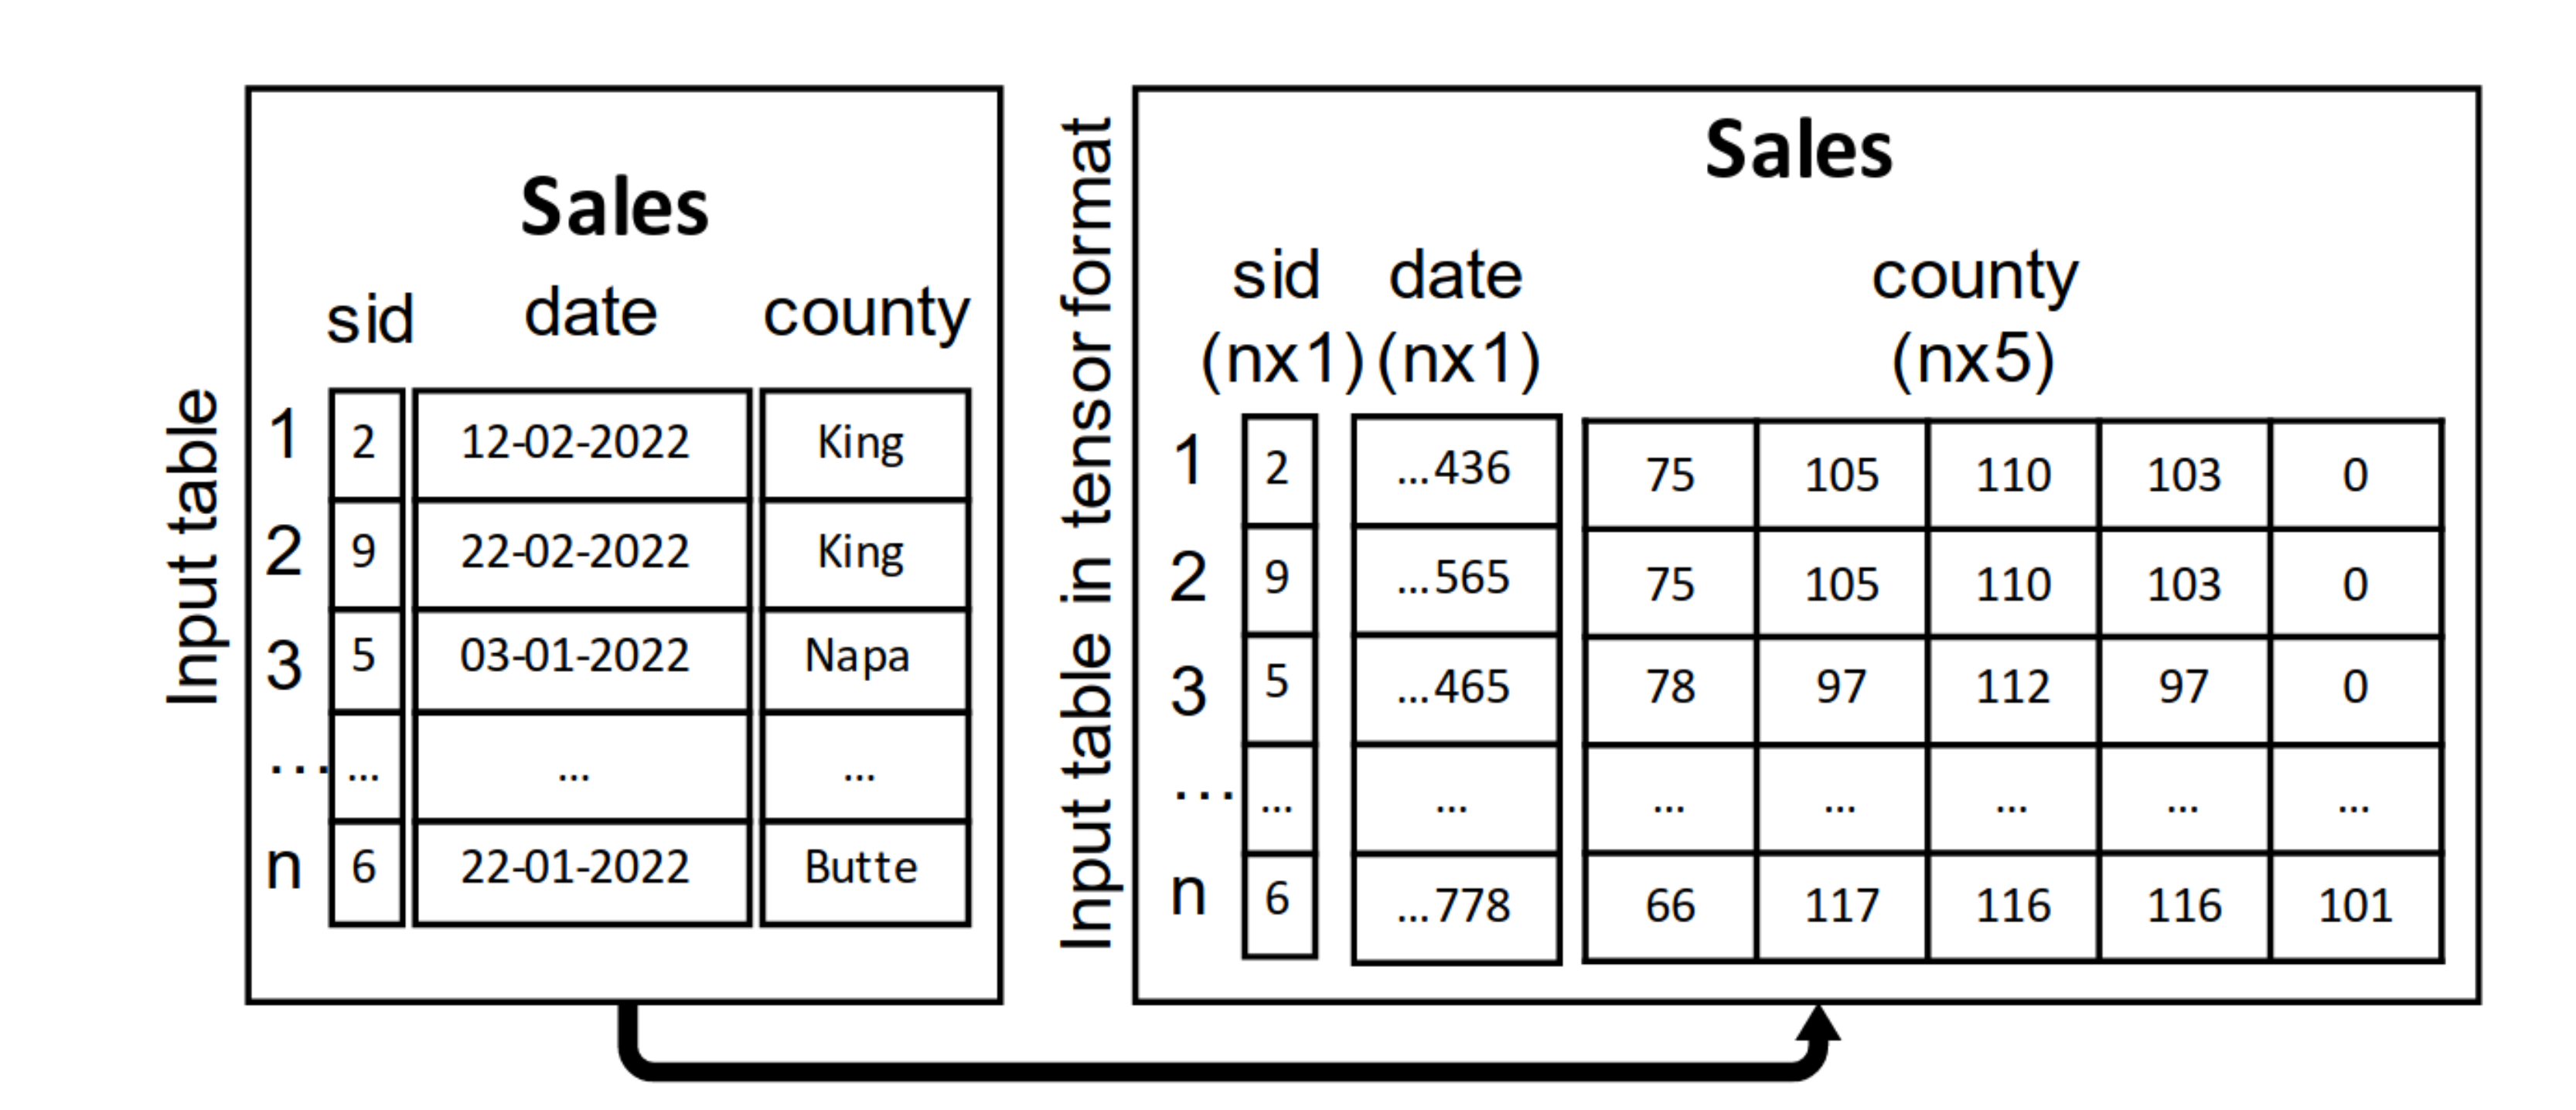
\includegraphics[width=0.9\linewidth]{otherPaper}
		\caption{TQP represents input tables in a columnar format with a 2d-tensor per column. Figure and caption from \cite{he2022query}.}
		\label{fig:otherpaper}
	\end{figure}

\subsubsection{Query Implementation}
	
	Unlike the query pattern matching found in TCUDB, the TQP paper presents a multilevel compilation hierarchy: A supplied SQL query is first compiled to an intermediate representation used for optimization before being compiled to a tree of tensor operations that can be mapped to a supported backend (ONNX, TVM, PyTorch, TorchScript).
	
	The chosen data representation format means that the the operators introduced in TCUDB do not work in TQP. The TQP authors show how traditional database algorithms such as sort based joins can be mapped to tensor operators. 
	
	We will take a look at two examples:
	
	\paragraph{Filtering}
	Simple filtering can be achieved using a bitmap operation. For this a tensor operation comparing given attributes sets a bitmap. In a second step the bitmap is used as a mask in a tensor masked-selection operation. 

	\paragraph{Joins}
	
	The paper presents a sort and hash based join; both work similar to their CPU counterparts. We note that as they do not directly invoke any calls to tensor cores but rather delegate this to the underlying framework. It is unclear wether the join is fully performed on the tensor core compared to TCUDB as operations such as \texttt{torch.sort} might not use a tensor core backend but run on CUDA cores.
	
	\subsection{Concluding Remarks on Related Work}
	
	TCUDB presents one of the first methods for using Tensors Cores in database workloads and presents novel approaches for modeling query operators as matrix multiplications, whereas related work focuses on using established algorithms (sort-based joins etc.) on CUDA \cite{yuan2013yin} or Tensor Cores \cite{he2022query}. Although TQP provides a different approach on using tensor cores 
	
	\section{Performance Evaluation} \label{sec:perf_eval}
	

	\subsection{Synthetic Benchmarks}
	
	First, we will look at a synthetic performance evaluation running the following snippet on a database of $x$ rows with $y$ distinct attributes per column.
	\begin{verbatim}
SELECT SUM(A.VAL), B.VAL
FROM A, B WHERE A.ID = B.ID
GROUP BY B.VAL
	\end{verbatim}

\paragraph{Fixed Number of Distinct Attributed Per Column}
Assume we have 32 distinct elements for every column and vary the number of rows in our table.
	In this case we expect the encoded table matrices to have 32 columns which would give TCUDB an inherent advantage over YDB and MonetDB. This is exactly what we can observe in Figure \ref{fig:bench1}, although they all scale geometrically TCUDB already starts in a better position giving TCUDB an exponential advantage as the number of rows doubles. 
	\begin{figure}
		\centering
		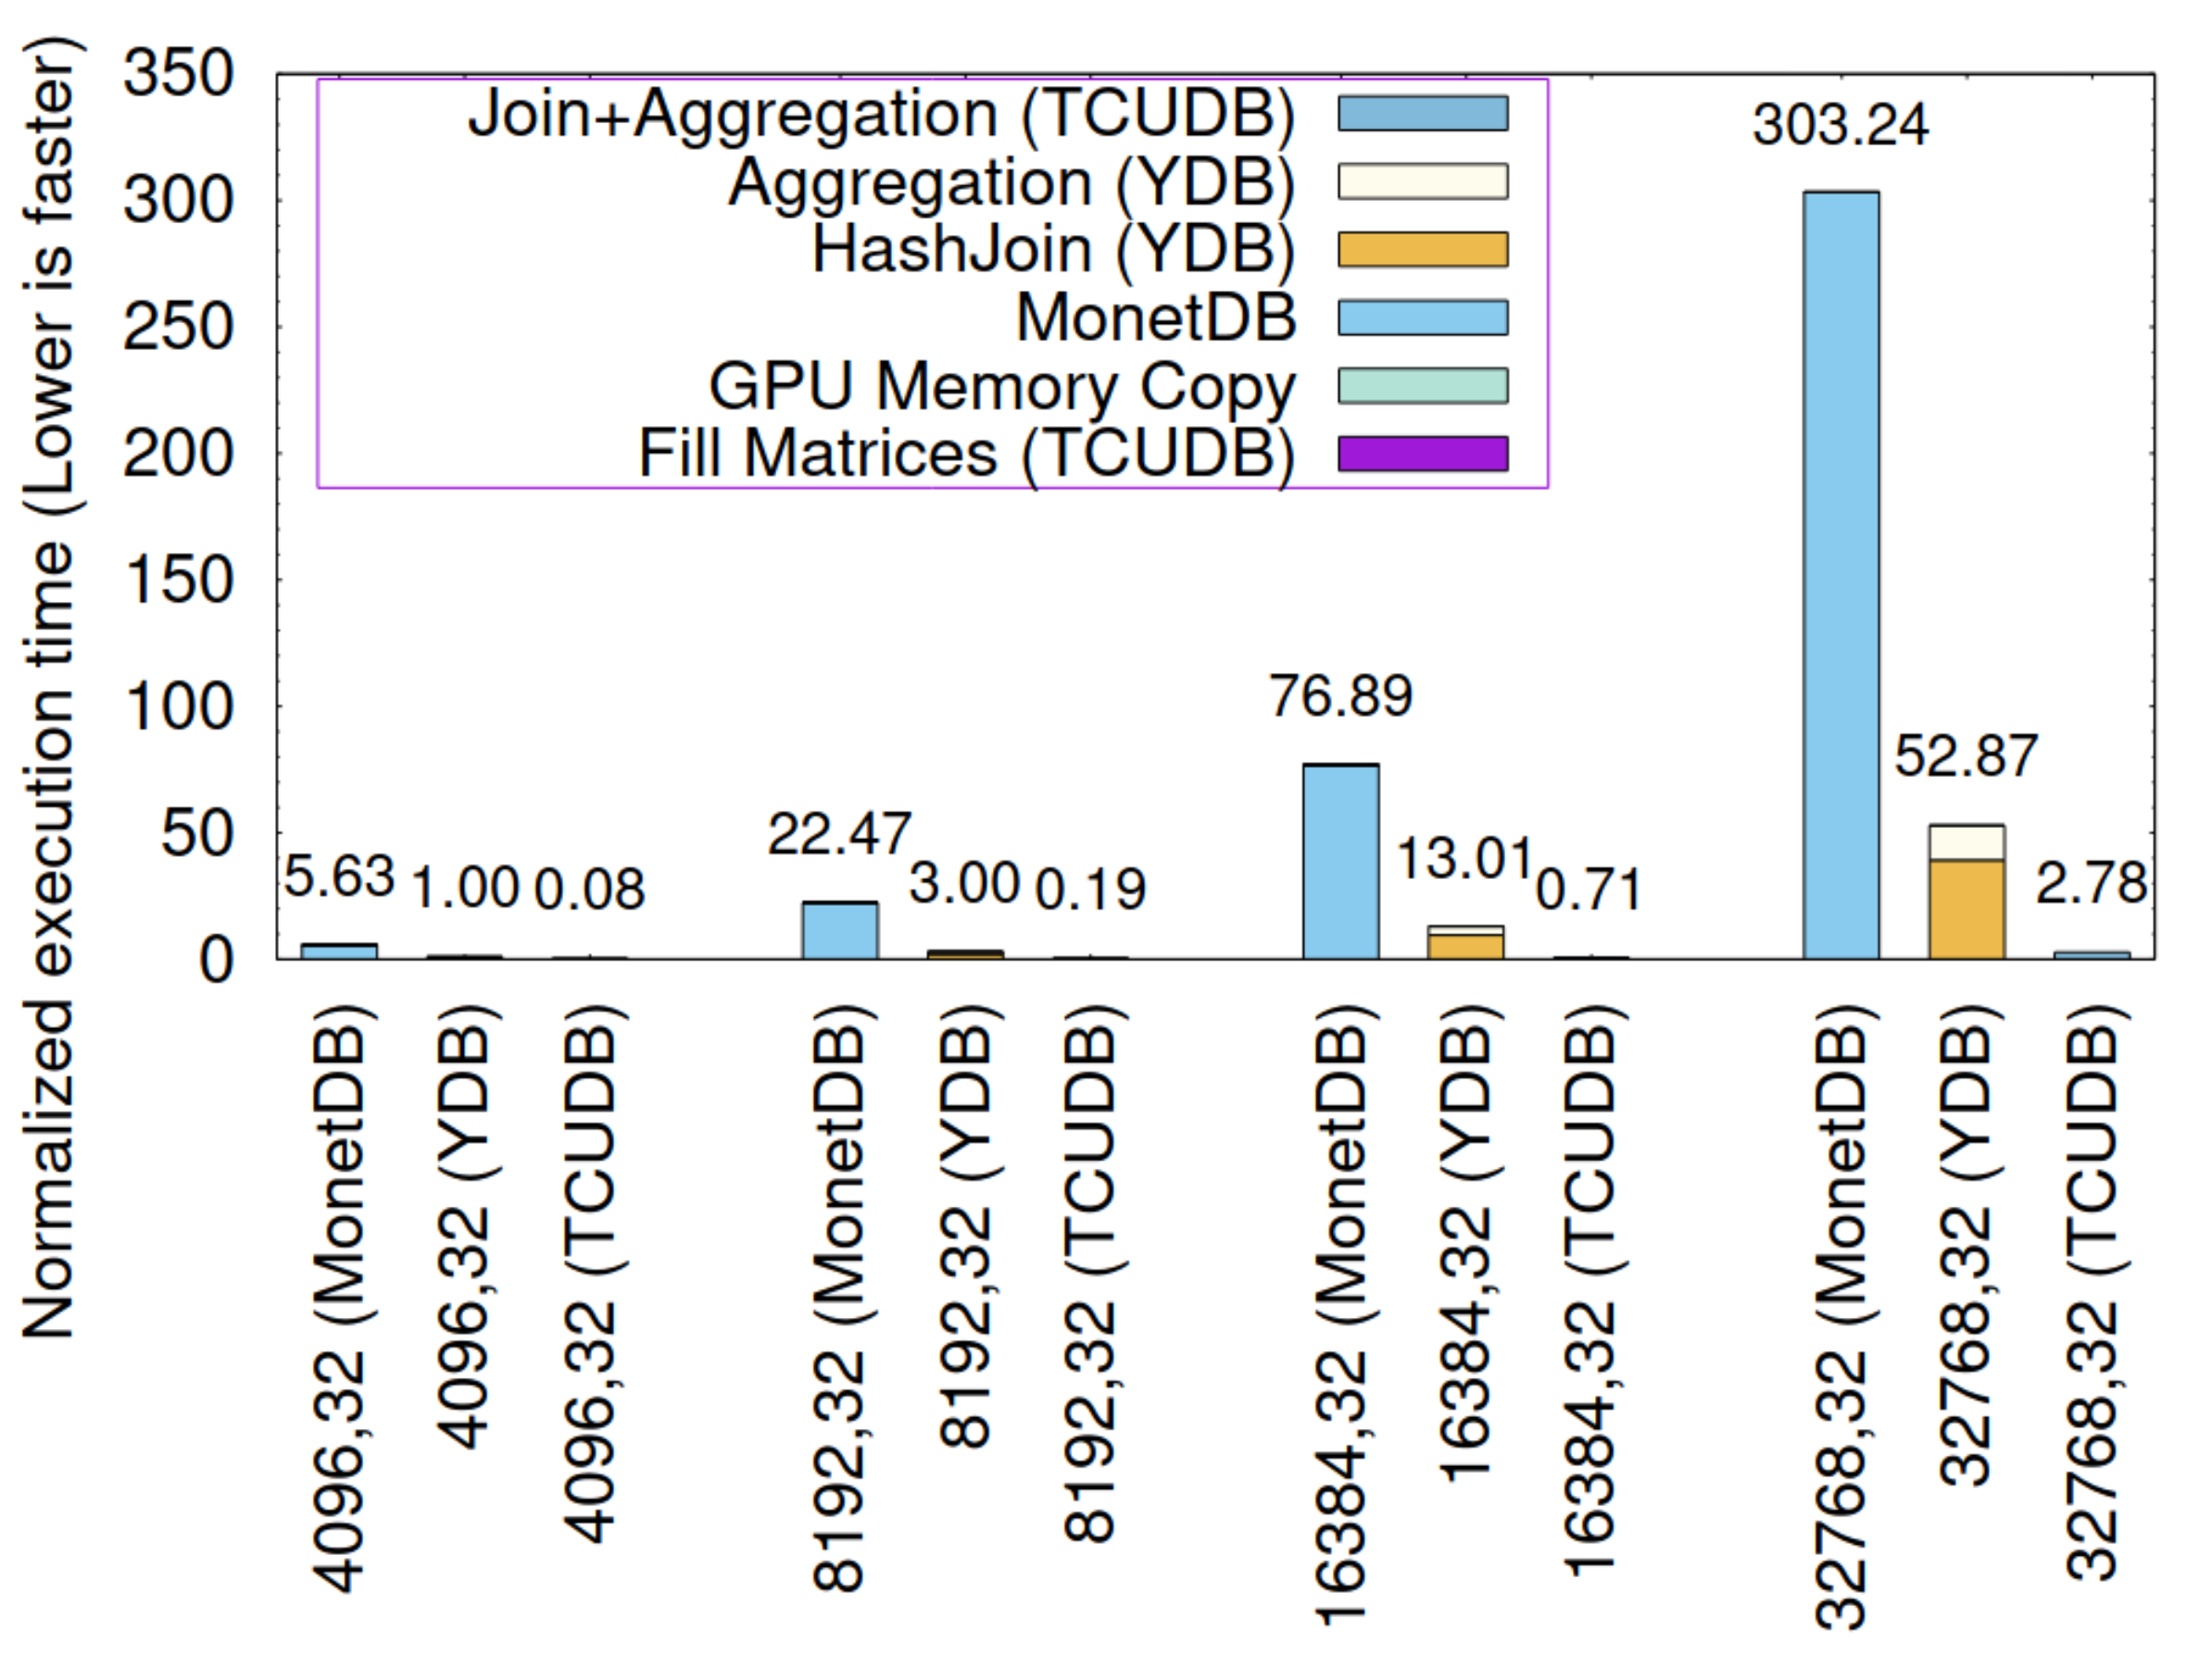
\includegraphics[width=0.9\linewidth]{bench1}
		\caption{Relative execution time with various number of records and 32 distinct values in target attribute. Figure and caption from \cite{hu2021tcudb}.}
		\label{fig:bench1}
	\end{figure}
	
\paragraph{Fixed Number of Distinct Attributed Per Column}
Note that in the previous case the matrix had 32 columns. If we drop this and now assume that we have a fixed number of rows, 4096 rows we can investigate how the number of distinct values per column influences TCUDB's runtime. Results can be seen in Figure \ref{fig:bench2}. Figure \ref{fig:bench2} shows as expected that the runtime for our tensor based processing increases linearly with $\Omega$(\#rows) as the matrix representing a table needs as many columns as there are individual attributes in a certain table column. Furthermore, we also witness that MonetDB gets faster as the number of distinct elements grows and even surpases TCUDB at a certain point. We conjecture that this stems from the individual hash buckets in the hash-based join getting smaller as the number of distinct elements increases.

		\begin{figure}
		\centering
		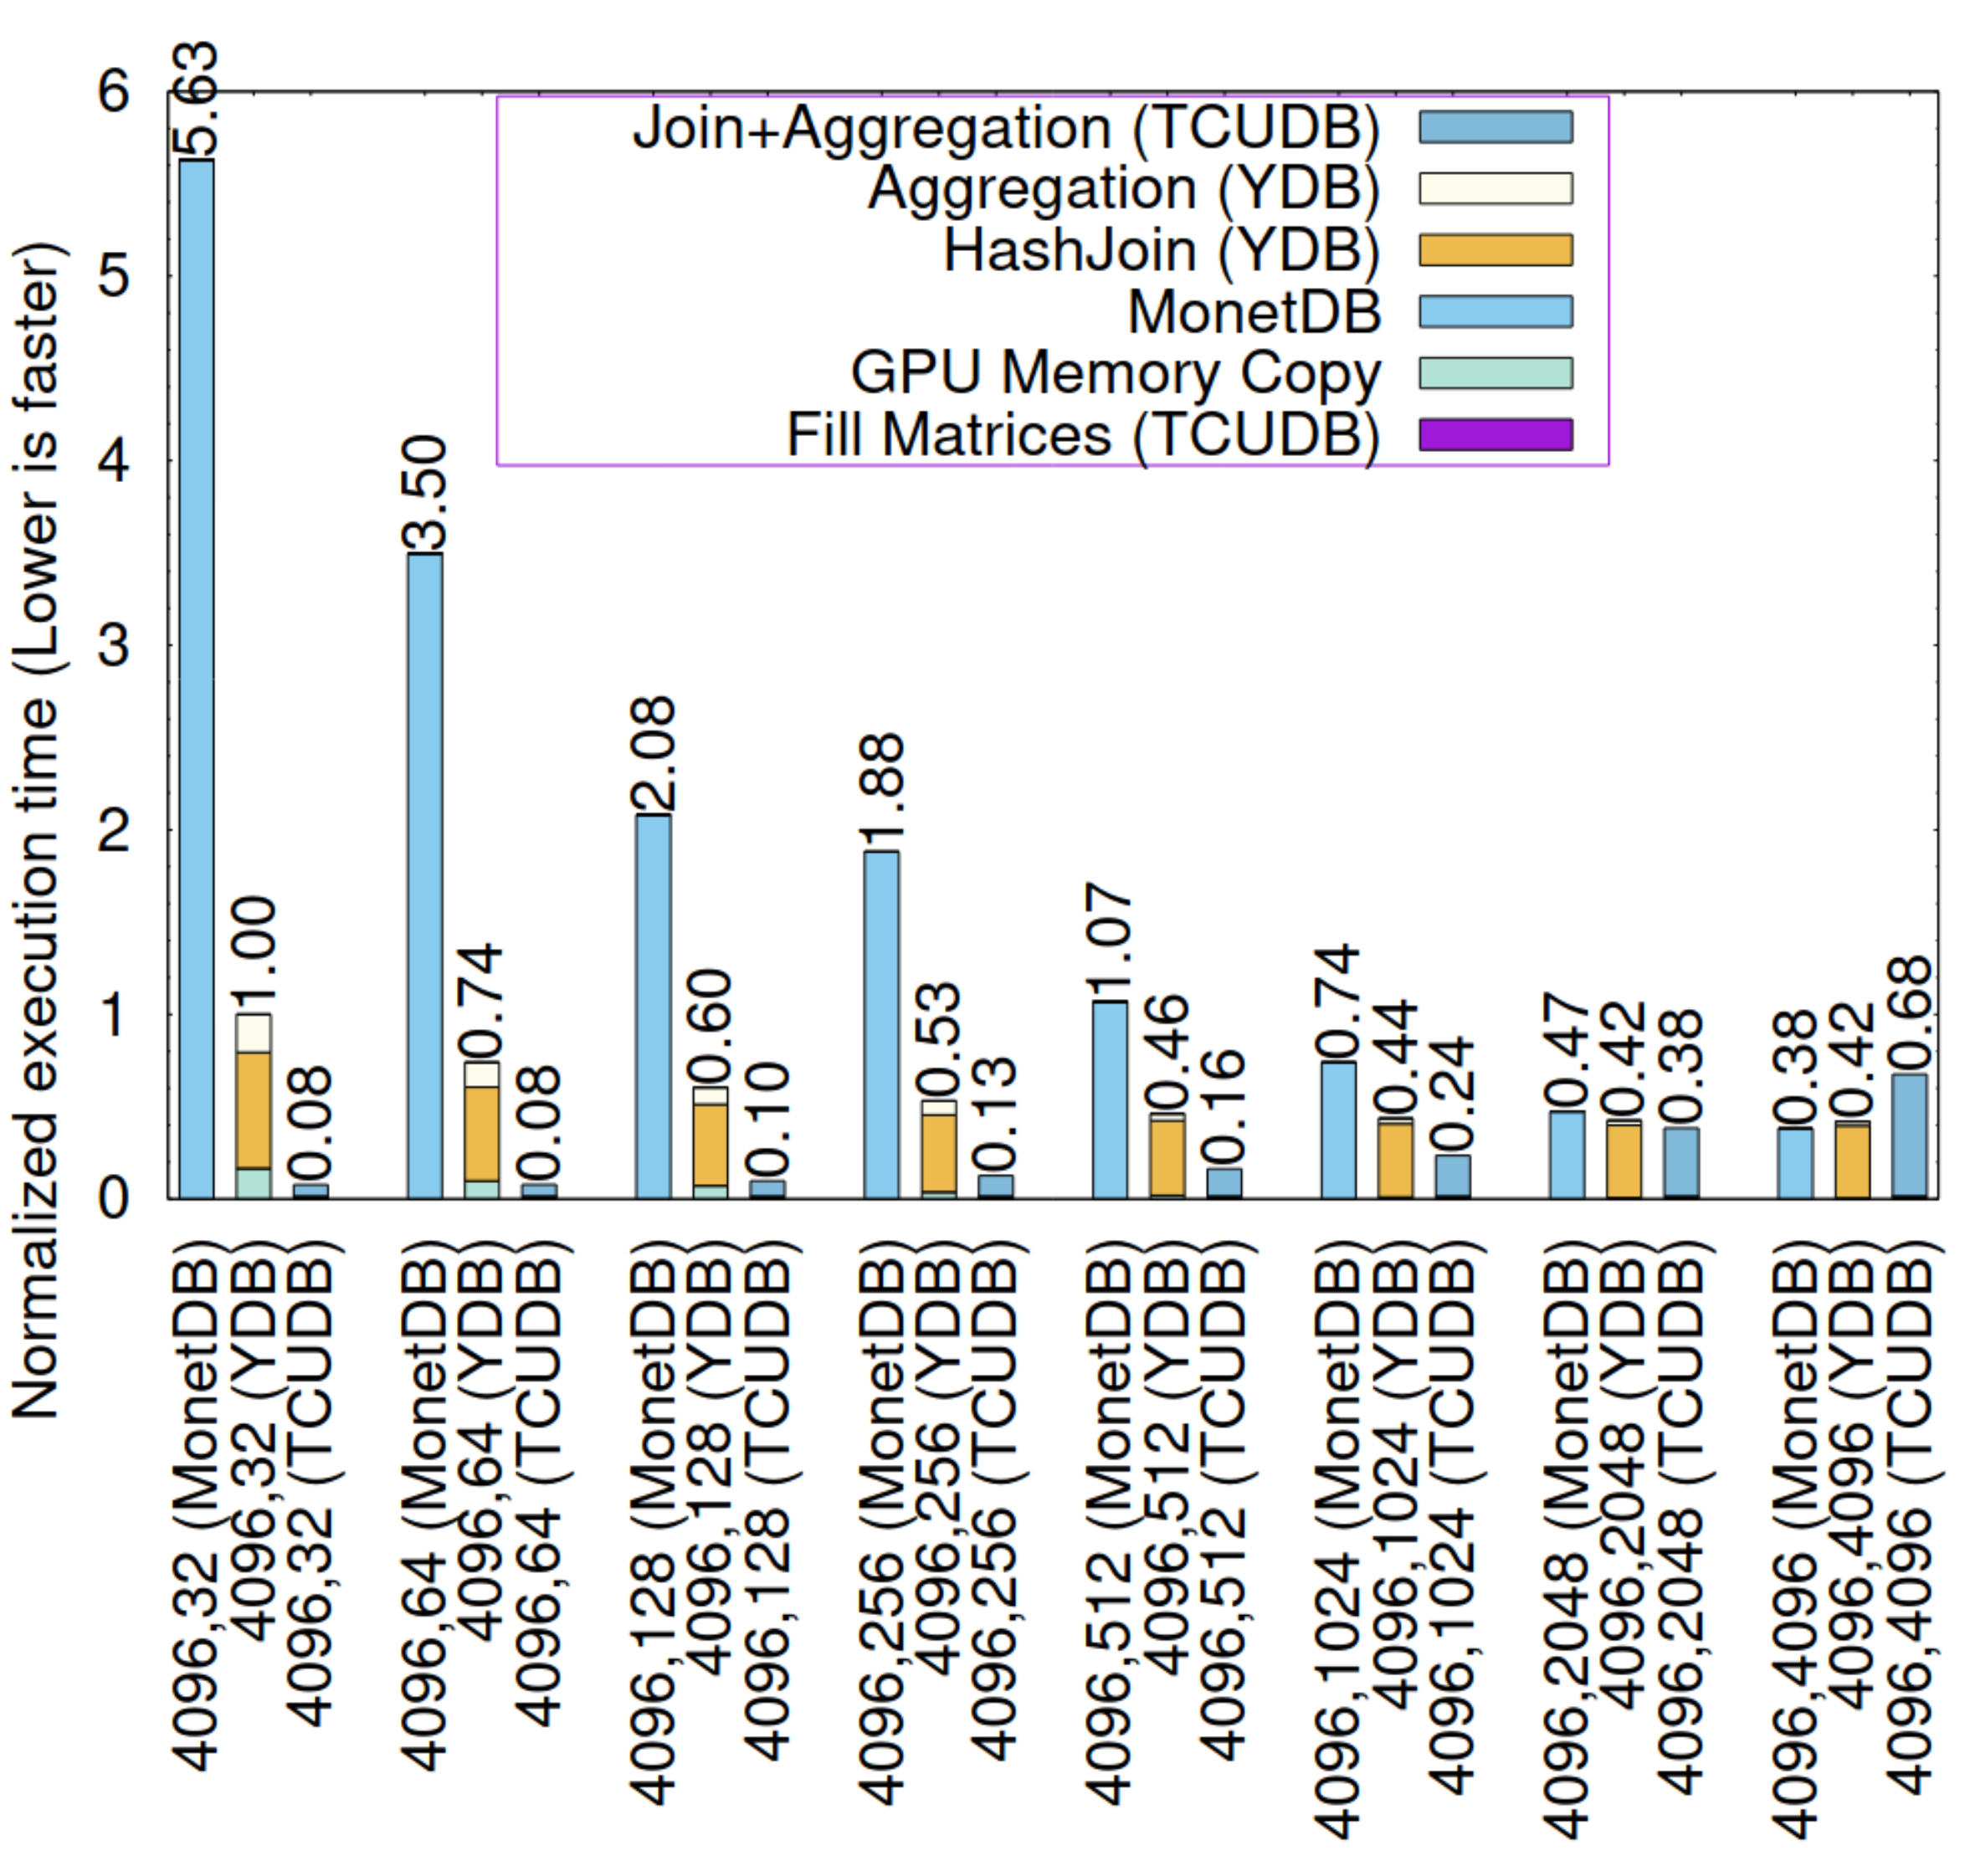
\includegraphics[width=0.9\linewidth]{bench2}
		\caption{Relative execution time with 4096 records and various distinct values in target attribute. Figure and caption from \cite{hu2021tcudb}.}
		\label{fig:bench2}
	\end{figure}
	
	\subsection{Star Schema Benchmark}
	
	\subsection{PageRank Benchmark}
	
	
	very expected
	
	cannot compare to the He paper.
	
	

	\begin{figure}
		\centering
		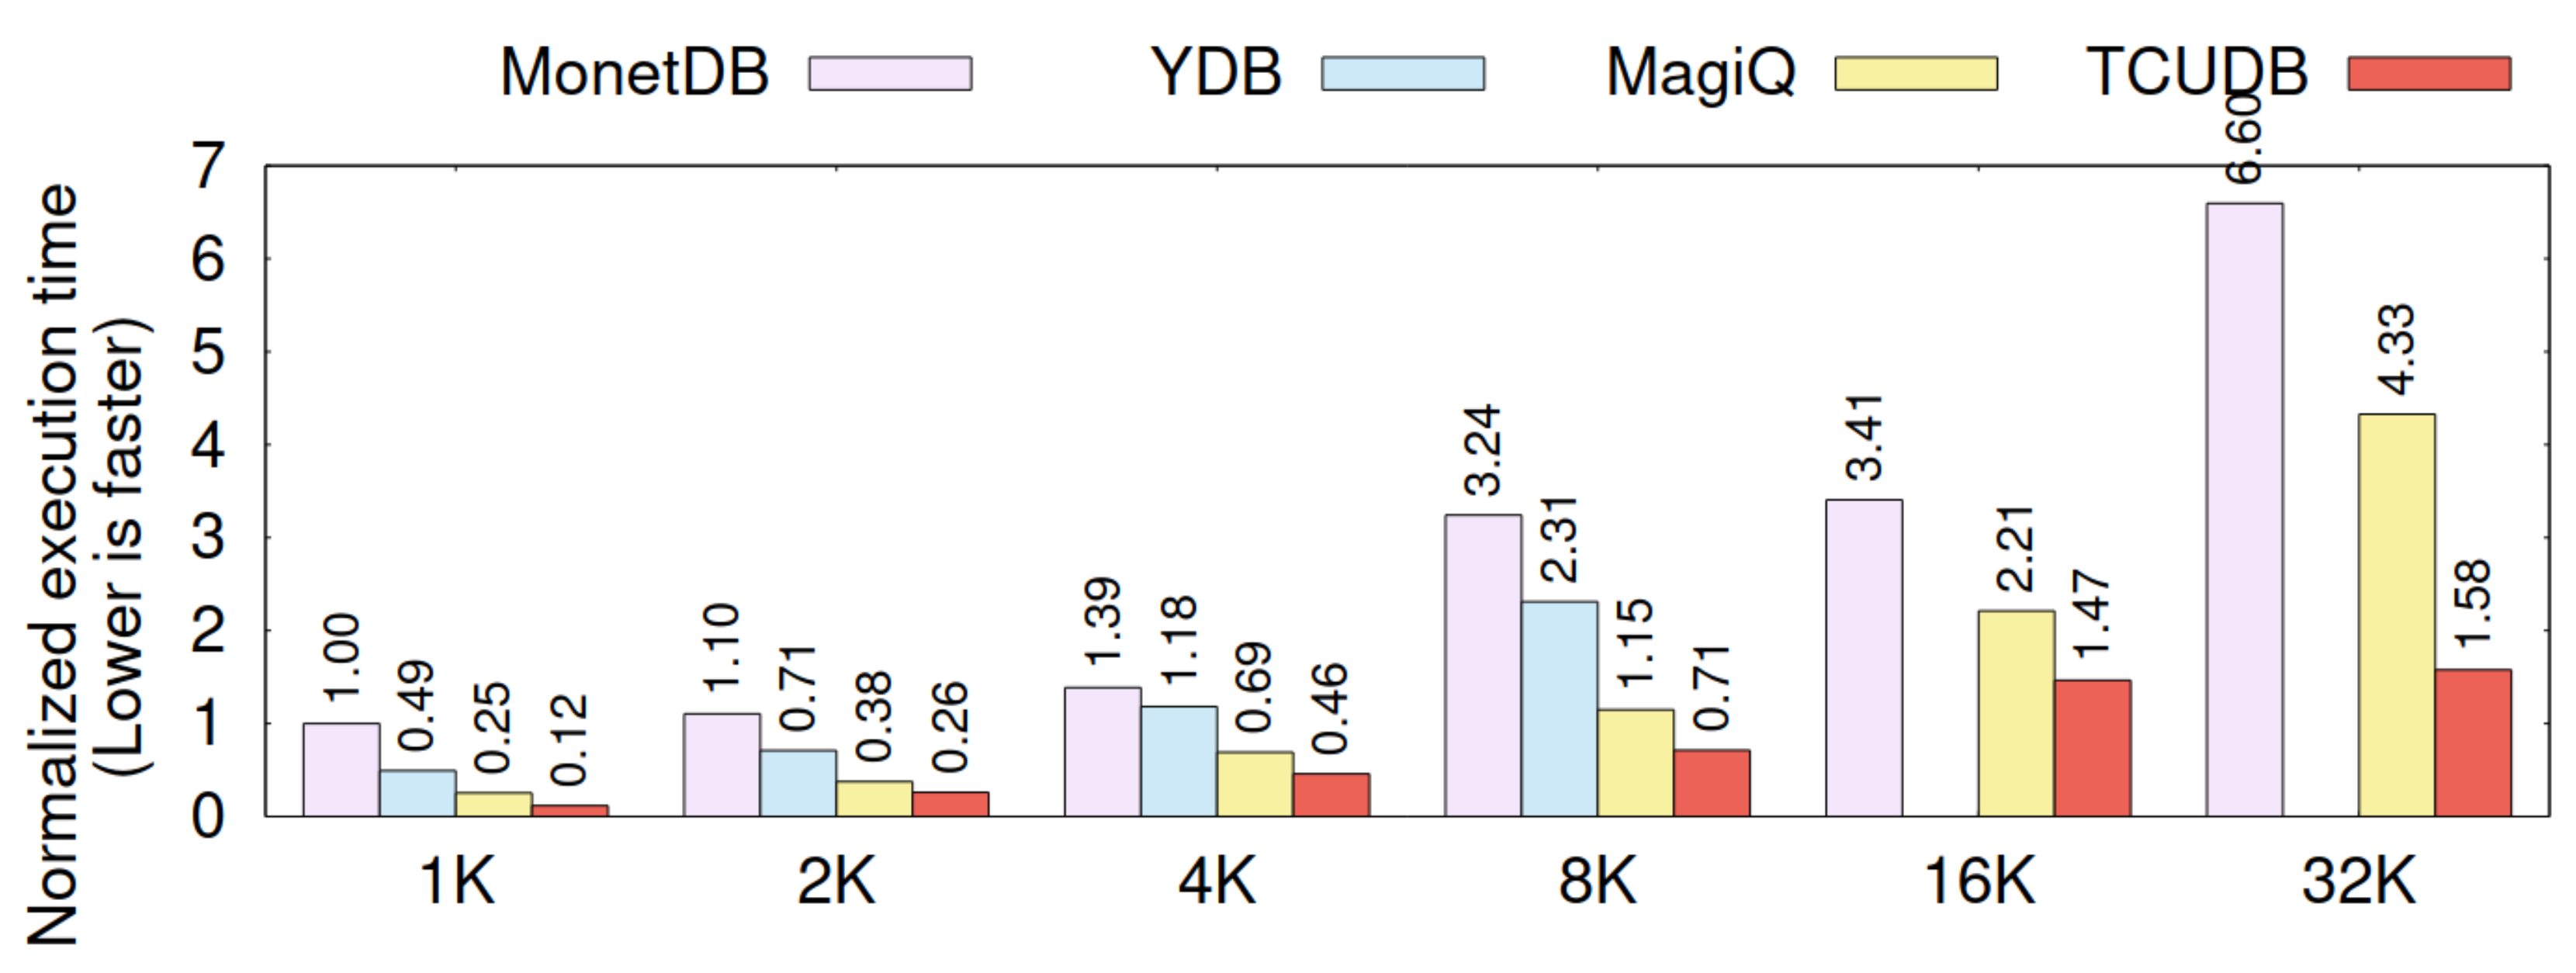
\includegraphics[width=0.9\linewidth]{bench3}
		\caption{The relative latency of the core join and aggregation operation when running PageRank. Figure and caption from \cite{hu2021tcudb}.}
		\label{fig:bench3}
	\end{figure}
	
	
	\begin{figure}
		\centering
		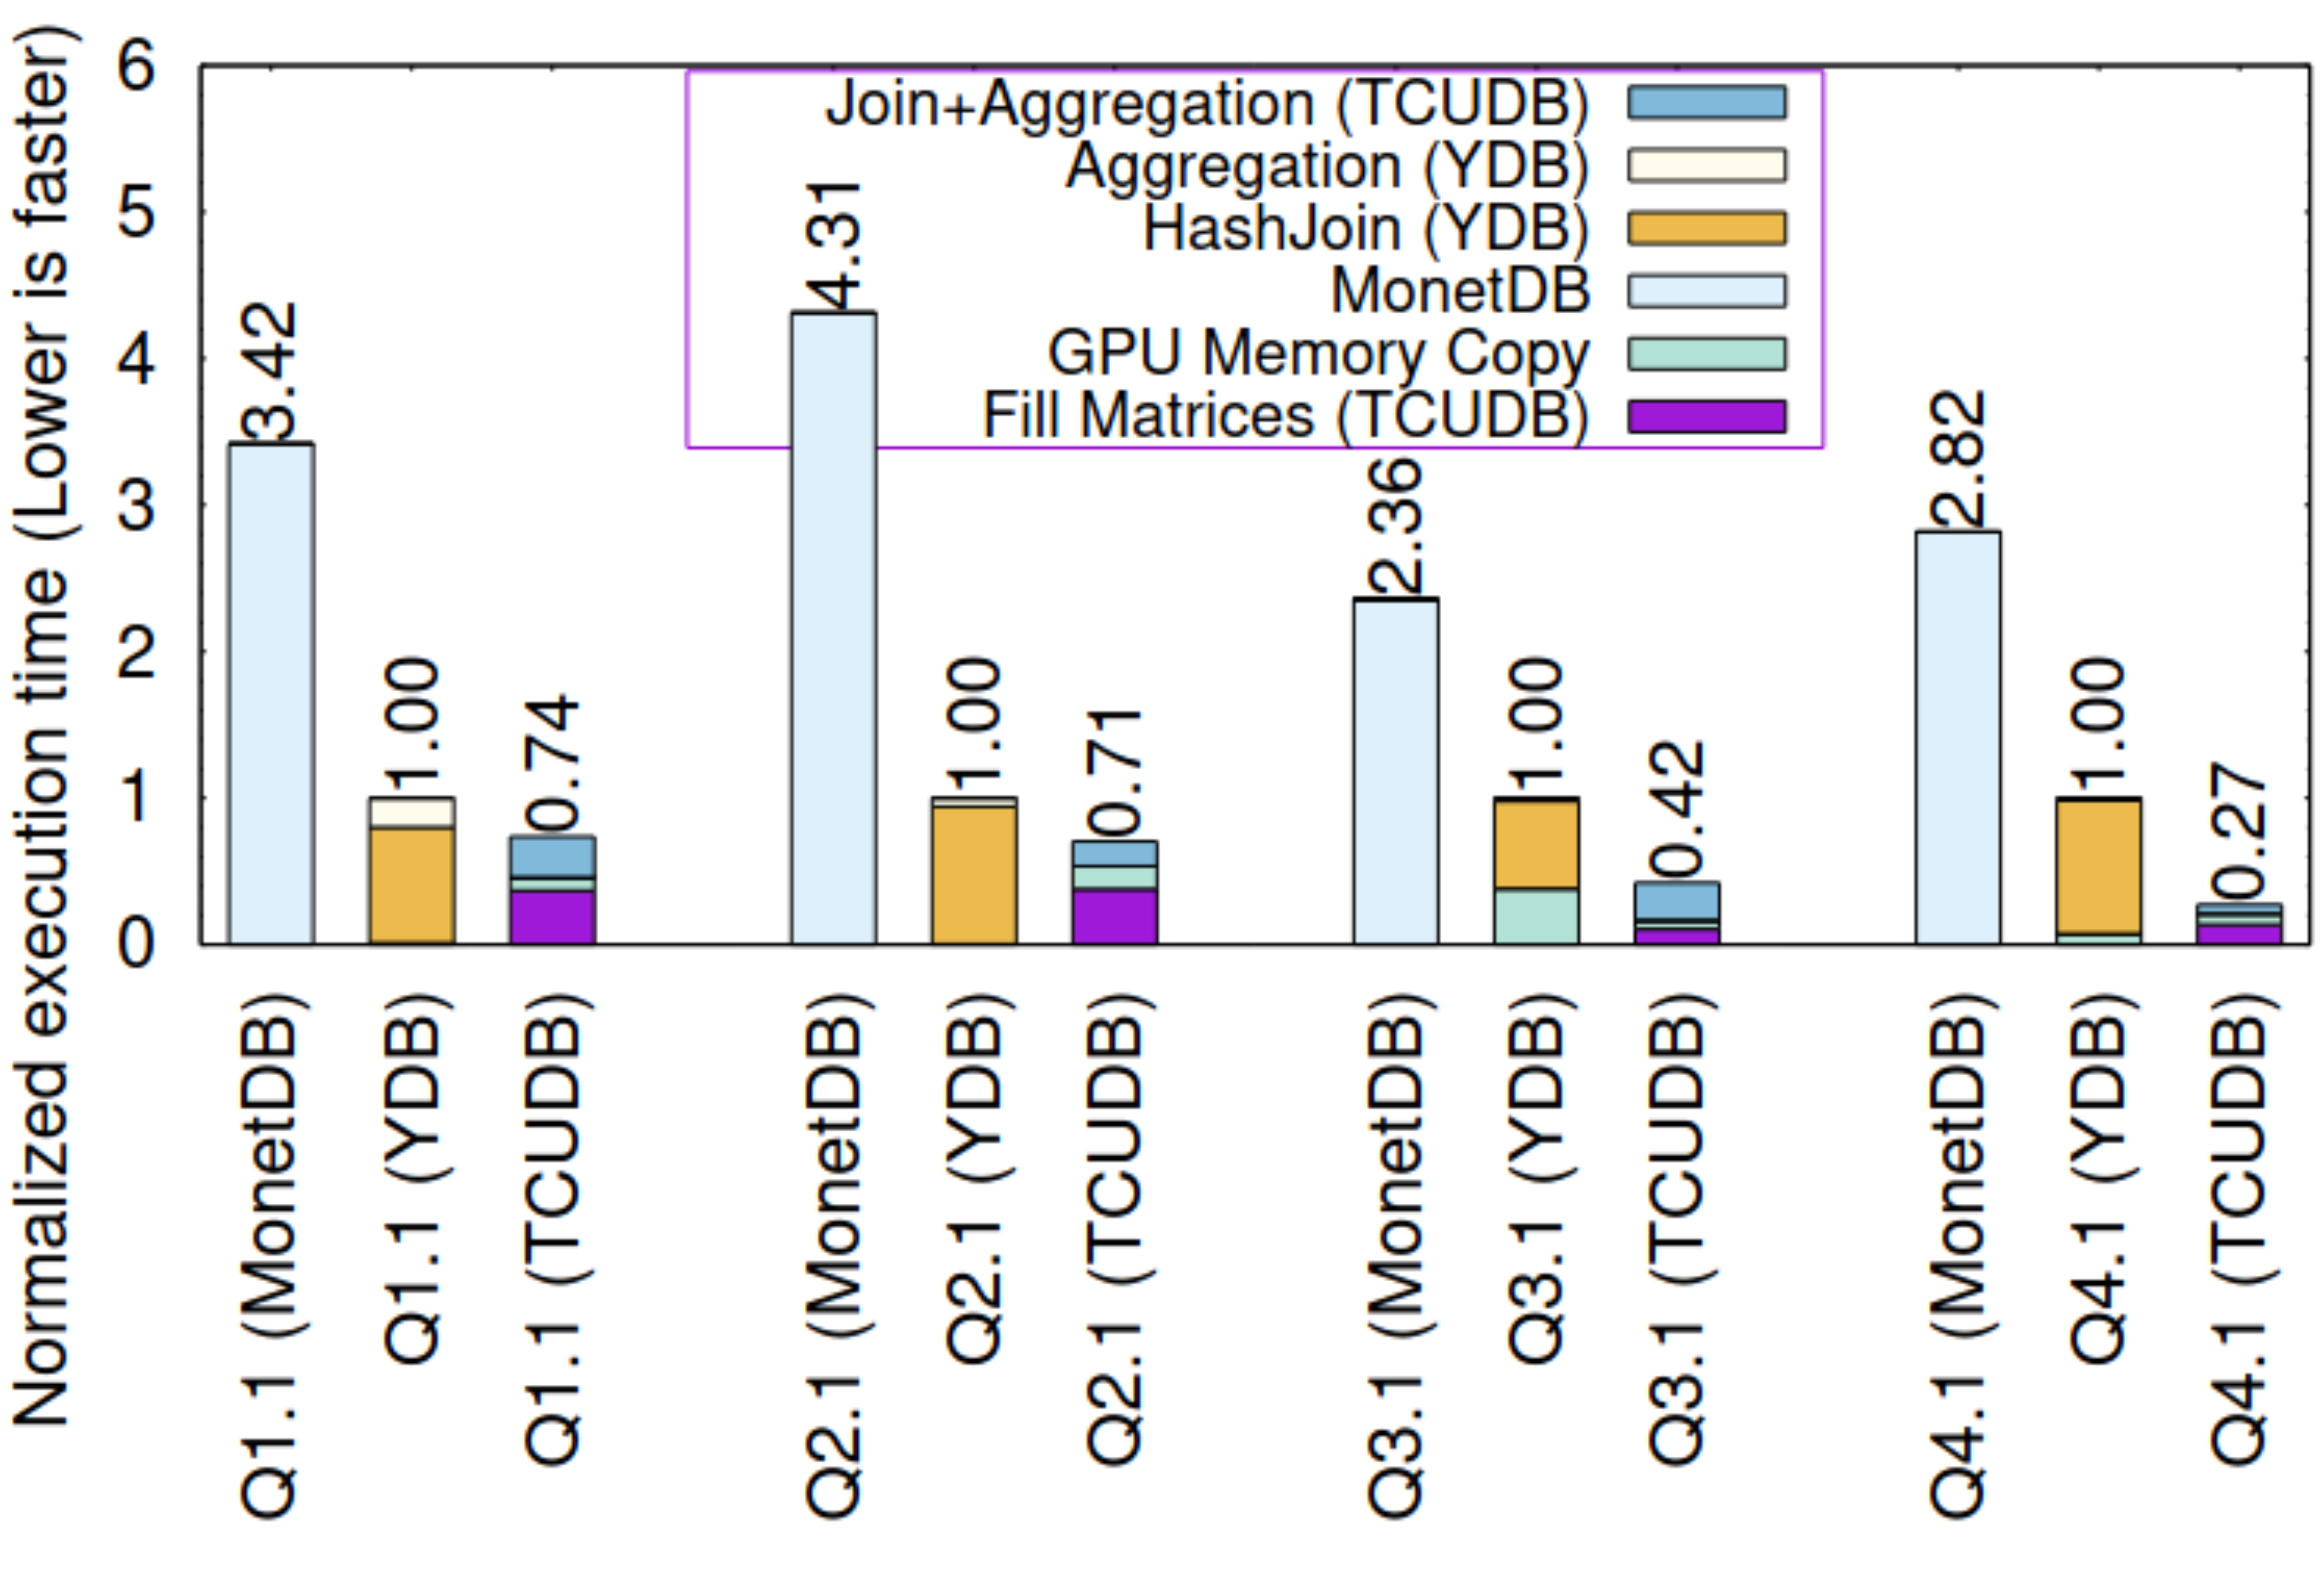
\includegraphics[width=0.9\linewidth]{bench4}
		\caption{The relative runtime of star  TODO schema benchmark on TCUDB compared to MonetDB and YDB running the same query as the baseline with scaling factor 1.}
		\label{fig:bench4}
	\end{figure}
	
	
	\section{Shortcomings}
	
	monetDB is super old, why not compared to Vectorwise, questionable 
	
	TPC-H benchmark like others
	
	TQP actualy uses tensor?? uses underlying
	
	clearly inefficient? 
	
	how many runs, average?
	
	
	\section{Conclusion}
	
\bibliographystyle{plain}
\bibliography{bibliography}
	

\end{document}
